\section{Билет 30. Потенциал двойного слоя. Интеграл Гаусса. Скачок потенциала двойного слоя при переходе через границу, на которой задаётся плотность}
% Затехал: Леонтьев Семён 377 группа

Пусть $\Gamma$ - граница класса $C^2$ ограниченной области $\Omega \subset \R^3$.

\begin{definition}
Функция вида
$V^{(2)}(x) = \int\limits_{\Gamma} \, \frac{\partial}{\partial \bar{n}_y}\roundBr{\frac{1}{\abs{x-y}}}\nu(y) dS_y $
называется \textit{\text{потенциалом двойного слоя}}
\end{definition}

Сразу будет удобно переписать определение в иной форме:
$$ \frac{\partial}{\partial \bar{n}_y}\roundBr{\frac{1}{\abs{x-y}}} = \sum_{k=1}^3 n_k(y)\frac{\partial}{\partial y_k}\frac{1}{\abs{x-y}} = \sum_{k=1}^3 \frac{n_k(y)(x_k - y_k)}{\abs{x-y}^3} = \frac{(x-y, \bar{n}_y)}{\abs{x-y}^3} \Rightarrow $$
$$ \Rightarrow V^{(2)}(x) = \int\limits_{\Gamma} \, \frac{(x-y, \bar{n}_y)}{\abs{x-y}^3}\nu(y) dS_y $$

\begin{lemma} Пусть $\nu(x) \in C(\Gamma)$. Тогда:

\
а) $V^{(2)}(x)$ - гармоническая функция в в $x\in \R^3\backslash \Gamma$;

\
б) $\displaystyle V^{(2)}(x) = O\roundBr{\frac{1}{\abs{x}^2}}$ при $\abs{x} \rightarrow \infty$
\end{lemma}

\begin{proof}
\

а) $$ V^{(2)}(x) = \sum_{k=1}^3\int\limits_{\Gamma} 
\
\underbrace{n_k(y)}_{\substack{\in C(\Gamma)\\ \text{т.к.} \Gamma \in C^2}}
\underbrace{\nu(y)}_{\substack{\in C(\Gamma)\\ \text{по}\\ \text{условию}}} 
\
\underbrace{\frac{\partial}{\partial y_k} \frac{1}{\abs{x-y}}}_{\substack{-\frac{\partial}{\partial x_k} \frac{1}{\abs{x-y}}\\ \in C\roundBr{(\R^3\backslash\Gamma)\times\Gamma}}}dS_y
\
=
\
-\sum_{k=1}^3\frac{\partial}{\partial x_k} \int\limits_{\Gamma}
\
\underbrace{n_x(y)\nu(y)\frac{1}{\abs{x-y}}dS_y}_{\substack{\text{потенциал простого слоя с}\\  \mu = n_k\cdot\nu\in C(\Gamma)\\ \Downarrow\\ \text{является гармонической}\\ \text{функцией в } R^3\backslash\Gamma}} 
 $$
 Остаётся воспользоваться тем, что производная гармонической функции - гармоническая.
\

б) Возьмём сразу сферу радиуса $R$ такую, что $\Gamma$ лежит внутри сферы. При $$\abs{x} \rightarrow \infty \Rightarrow \abs{x}>2R \Rightarrow
\abs{y} \leq \frac{\abs{x}}{2} \Rightarrow \abs{x-y}^2\geq \roundBr{\abs{x} - \abs{y}}^2 \geq \frac{\abs{x}}{4}  $$
$$\abs{\frac{\partial}{\partial\bar{n}_y} \frac{1}{\abs{x-y}}} \leq \frac{\abs{x-y}\cdot\abs{\bar{n}_y}}{\abs{x-y}^3} = \frac{1}{\abs{x-y}^2} \Rightarrow$$
$$\Rightarrow\abs{V^{(2)}(x)} = \abs{\int\limits_{\Gamma} \, \frac{\partial}{\partial \bar{n}_y}\roundBr{\frac{1}{\abs{x-y}}}\nu(y) dS_y}\leq\frac{4}{\abs{x}^2}\int\limits_{\Gamma} \, \abs{\nu(y)}dS_y\leq4\norm{\nu(y)}_{C(\Gamma)}\int\limits_{\Gamma} dS_y\cdot\frac{1}{\abs{x}^2 \Rightarrow}$$
$$\Rightarrow V^{(2)}(x) = O\roundBr{\frac{1}{\abs{x}^2}} \text{при} x\rightarrow \infty$$
\end{proof}

\begin{lemma}
Если $\Omega$ ограниченная область с границей $\Gamma \in C^2$, то $\forall x,y\in\Gamma, x\neq y$, справедлива оценка $$\abs{\frac{(x-y,n(y))}{\abs{x-y}^2}}\leq\frac{M}{\abs{x-y}}$$
\end{lemma}
\begin{proof}
Пусть $d$ - число из определения поверхности с границей $\Gamma \in C^2$:
\begin{itemize}[noitemsep]
\item если $\displaystyle  \abs{x-y}\geq d$, то $\displaystyle \frac{\abs{(x-y,\bar{n}_y)}}{\abs{x-y}^3} \leq \frac{1}{\abs{x-y}^2} \leq \frac{1}{d}\frac{1}{\abs{x-y}}$
\item если $\abs{x-y} < d$, то свяжем $y$ с локальной системой координат. В этой системе: 
\

$\displaystyle y=(0,0,0)$, $x = (\xi_1,\xi_2, F(\xi_1, \xi_2))$, $\bar{n}_y = (0,0,1) \Rightarrow$
\

 $\displaystyle \abs{x-y, \bar{n}_y)} = \abs{F_y(\xi_1, \xi_2)} \leq M_2(\xi_1^2+\xi_2^2)\leq M_2(\xi_1^2+\xi_2^2 + F_y^2(\xi_1, \xi_2) = M_2\abs{x-y}^2$, что и требовалось.
\end{itemize}
\end{proof}
\begin{lemma}
Пусть $\nu(x) \in C(\Gamma)$. Тогда потенциал двойного слоя $V^{(2)} \in C(\Gamma)$
\end{lemma}

\begin{proof}
Используем признак полярного ядра (билет №24). В силу леммы $\abs{K(x,y)} \leq \frac{M}{\abs{x-y}}$ и 
\
$K(x,y) = \displaystyle \frac{(x-y, \bar{n}_y)}{\abs{x-y}^2}\in C\roundBr{(\Gamma\times\Gamma)\backslash \curlyBr{x=y}}$
Оператор с полярным ядром переводит непрерывные функции в непрерывные, а $\nu \in C(\Gamma) \Rightarrow V^{(2)}(x)\in C(\Gamma)$

\end{proof}
Наша цель - описать скачок $V^{(2)}(x)$ при переходе через границу. Для этого потребуется несколько вспомогательных утверждений.
\begin{lemma}
Пусть $\Omega$ - ограниченная область с границей $\Gamma\in C^2$. Тогда интеграл $\displaystyle V^{(2)}_{GAUSS}(x) = 
\int\limits_{\Gamma} \frac{\partial}{\partial\bar{n}_y}\roundBr{\frac{1}{\abs{x-y}}}\nu(y) \cdot 1 \cdot dS_y = \dfrac{(x-y, \bar{n}_y)}{\abs{x-y}^3} dS_y$ - (интеграл Гаусса) равен 

$\begin{cases} -4\pi, x\in \Omega \\
-2\pi, x\in \Gamma \\ 0, x\in\R^3\backslash \overline{\Omega}
\end{cases}$
\end{lemma}

\begin{proof}
1) Пусть $x \in \Omega$. Возьмём $u(x)\equiv 1$ и запишем представление этой функции в виде суммы трёх потенциалов:
$$u(x) \equiv 1 = \int\limits_{\Omega} \roundBr{\frac{-1}{4\pi\abs{x-y}}}\underbrace{\Delta 1}_{\substack{ = 0}} dy + \int\limits_{\Gamma}\frac{\partial}{\partial \bar{n}_y}\roundBr{\frac{-1}{4\pi\abs{x-y}}}u(y)dS_y - \int\limits_{\Gamma}\roundBr{\frac{-1}{4\pi\abs{x-y}}}
\
\underbrace{\frac{\partial u(y)}{\bar{n}_y}}_{\substack{ = 0}}
\
=
\
-\frac{1}{4\pi}V_{GAUSS}^{(2)}(x)
$$
2) Пусть $x \in \R^3\backslash \overline{\Omega}$ 
Возьмём $u(y) \equiv 1$ и $v(y) = \frac{1}{\abs{x-y}}$ и воспользуемся для этих функций первой формулой Грина:
$$\int\limits_{\Omega} \underbrace{\Delta_y v(y)}_{\substack{ = 0}} \cdot u(y)dy = \underbrace{\int\limits_{\Gamma}\frac{\partial}{\partial \bar{n}_y}v(y)u(y)dS_y}_{\substack{ = V_{GAUSS}^{(2)}(x)}}
-
\underbrace{\int\limits_{\Omega}\roundBr{\nabla_y v(y), \nabla 1}dy}_{\substack{ = 0}}
\Rightarrow
V_{GAUSS}^{(2)}(x) = 0
$$
3) Пусть $x\in \Gamma$. Введём $B = B(x,\varepsilon), \Omega_\varepsilon = \Omega\backslash\bar{B}, \Gamma_\varepsilon = \Gamma\backslash B, \sigma_\varepsilon = \partial B\cap \bar{\Omega} $
Тогда $\partial \Omega_\varepsilon = \Gamma_\varepsilon \cup\sigma_\varepsilon \Rightarrow x\in \R^3 \backslash \bar{\Omega}_\varepsilon$
\begin{center}
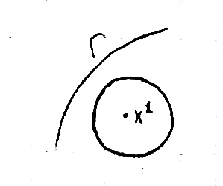
\includegraphics[width=0.2\textwidth]{30_1_new}
\end{center}
Согласно второму пункту можем написать $\displaystyle\int\limits_{\partial \Omega_\varepsilon}\dfrac{\partial}{\partial \bar{n}_y}\roundBr{\dfrac{1}{\abs{x-y}}} dS_y = 0$
Значит $$\underbrace{\int\limits_{\Gamma_\varepsilon} \frac{\partial}{\partial \bar{n}_y}\roundBr{\frac{1}{\abs{x-y}}} dS_y}_{\substack{\rightarrow \int\limits_{\Gamma} \text{при } \varepsilon \rightarrow 0}}
+
 \int\limits_{\sigma_\varepsilon} \frac{\partial}{\partial \bar{n}_y}\roundBr{\frac{1}{\abs{x-y}}} dS_y = 0 $$
 Покажем, что $$\displaystyle\int\limits_{\sigma_\varepsilon} \dfrac{\partial}{\partial \bar{n}_y}\roundBr{\dfrac{1}{\abs{x-y}}} dS_y \rightarrow 2\pi \text{ при } \varepsilon \rightarrow 0 \text{ } \dfrac{\partial}{\partial \bar{n}_y}\roundBr{\dfrac{1}{\abs{x-y}}} = \dfrac{(x-y, \bar{n}_y)}{\abs{x-y}^3} = \dfrac{\abs{x-y}\abs{\bar{n}_y}}{\abs{x-y}^3} 
=
\dfrac{1}{\abs{x-y}^2} = \dfrac{1}{\eps^2} $$
Поэтому $\displaystyle\int\limits_{\sigma_\varepsilon} \dfrac{\partial}{\partial \bar{n}_y}\roundBr{\dfrac{1}{\abs{x-y}}} dS_y = \dfrac{1}{\varepsilon^2}\int\limits_{\sigma_\varepsilon}dS_y$
\

При малых $\varepsilon$ кусок границы $\Gamma$ внутри $\rightarrow$ к полуплоскости $\Rightarrow \sigma_\varepsilon \rightarrow$ к полусфере.
\

Поэтому  $\int\limits_{\sigma_\varepsilon}dS_y = 2\pi\varepsilon^2\roundBr{1+O(1)}$, что и требовалось
\end{proof}

$\bf{Offtop:}$ Геометрический смысл интеграла Гаусса: 
$\dfrac{(y-x, \bar{n}_y)}{\abs{x-y}^3}dS_y = \dfrac{dS_ycos\beta}{\abs{x-y}^2} = d\Omega$
\begin{center}
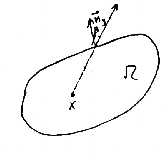
\includegraphics[width=0.2\textwidth]{30_2_new}
\end{center}

-- телесный угол, под которым из точки $x$ видна часть $dS_y$. Интеграл Гаусса есть сумма всех таких углов со знаком $"\text{минус}"$. Поэтому геометрически последняя лемма очевидна.


\begin{lemma}
Пусть $\Omega$ - ограниченная область в $\R^3$  с границей $\Gamma \in C^2$. Пусть $x^o \in \Gamma$. Тогда
\

 $\forall x: (x\in \R^3)\cap\roundBr{\abs{x-x^o}<\dfrac{d_*}{2}} $ верно $\displaystyle\int\limits_{\abs{y-x^o}<d_*}\dfrac{(x-y, \bar{n}_y)}{\abs{x-y}^3}dS_y <K, d_* = \dfrac{1}{2}min\roundBr{d, \dfrac{2}{M_2}}
$
\

Без доказательства
\end{lemma}
\begin{lemma}
Пусть $\Omega$ - ограниченная область в $\R^3$ с границей $\Gamma \in C^2$. Пусть $x^o\in \Gamma$. Тогда 
$\displaystyle\lim_{x \to x^o} W(x, x^o) = W(x^o, x^o)$, где $W(x, x^o) = \displaystyle\int\limits_{\abs{y-x^o}<d_*}\dfrac{(x-y, \bar{n}_y)}{\abs{x-y}^3}\roundBr{\nu(y) - \nu(x^o)}dS_y$,  а $\nu(x)\in C(\Gamma)$
\end{lemma}

\begin{proof}
Требуется показать, что $ \forall \varepsilon>0 \Exists \delta_\varepsilon>0: \Forall x: \abs{x-x^o} < \delta_\varepsilon \rightarrow \abs{W(x,x^o) - W(x^o, x^o)} < \varepsilon.
$
Функция $\nu(x)$ непрерывна на компакте, следовательно она и равномерно непрерывна на нём. Значит 
$\exists \beta = \beta(\varepsilon): \Forall y \in \Gamma: \abs{y-x^o}<\delta \rightarrow \abs{\nu(y) - \nu(x^o)} <\varepsilon
$
. Выберем $\beta \leq \dfrac{d_*}{2}$
$$
\abs{W(x,x^o) - W(x^o,x^o)} = \abs{\displaystyle\int\limits_{\Gamma}\roundBr{\dfrac{(x-y, \bar{n}_y)}{\abs{x-y}^3} 
-
\dfrac{(x^o-y, \bar{n}_y)}{\abs{x^o-y}^3} }\roundBr{\nu(y) - \nu(x^o)}dS_y} 
\leq
$$
$$
\leq
\displaystyle\int\limits_{\abs{y-x^o}<\beta}\underbrace{\roundBr{\dfrac{(x-y, \bar{n}_y)}{\abs{x-y}^3} 
-
\dfrac{(x^o-y, \bar{n}_y)}{\abs{x^o-y}^3} }}_{\substack{\leq K+K}}
\underbrace{\roundBr{\nu(y) - \nu(x^o)}}_{\substack{\leq \varepsilon}}dS_y 
\
+$$ $$
\
\displaystyle\int\limits_{\Gamma\backslash\roundBr{\abs{y-x^o}<\beta}}\underbrace{\roundBr{\dfrac{(x-y, \bar{n}_y)}{\abs{x-y}^3} 
-
\dfrac{(x^o-y, \bar{n}_y)}{\abs{x^o-y}^3} }}_{\substack{\leq \psi(x); \psi(x^o) = 0 \\ 
\Downarrow \\
\exists \delta_1: \norm{\psi(x)}< \varepsilon,\\
\text{если} \abs{x-x^o} < \delta_1 
}}
\underbrace{\roundBr{\nu(y) - \nu(x^o)}}_{\substack{\leq 2\norm{\nu}_{C(\Gamma)}}}dS_y 
$$

Значит, при $\abs{x-x^o}\leq max \roundBr{\dfrac{d_*}{2}, \delta_1(\varepsilon)}$
имеет место оценка 
$\abs{W(x, x^o) - W(x^o, x^o)} \leq 2K\varepsilon + 2\varepsilon\norm{\nu}_{C(\Gamma)}
$
\end{proof}

Теперь можно перейти к описанию скачка потенциала.
\begin{theorem}
Пусть $\Omega$ - ограниченная область в $\R^3$ с границей $\Gamma \in C^2$, а $\nu(x) \in C(\Gamma)$. Тогда потенциал двойного слоя $V^{(2)}(x) \in C(\bar{\Omega})$ и $V^{(2)}(x) \in C(\R^3\backslash\bar{\Omega})$ (можно непрерывно продолжить на замыкания). Обозначим $\forall x^o\in \Gamma: V^{(2)}_+(x^o) = \displaystyle \lim_{x\in \Omega,  x\to x^o} V^{(2)}(x);
V^{(2)}_-(x^o) = \displaystyle \lim_{x\in \R \backslash \bar{\Omega},  x\to x^o} V^{(2)}(x) $ 
Тогда $V^{(2)}_\pm(x^o) = V^{(2)}(x^o) \mp 2\pi\nu(x^o)$
\end{theorem}

\begin{proof}
$$V^{(2)}(x) = W(x, x^o) + \nu(x^o) \int\limits_{\Gamma} \, \frac{(x-y, \bar{n}_y)}{\abs{x-y}^3}\nu(y) dS_y$$
$$ V^{(2)}_+(x^o) = \displaystyle \lim_{x\in \Omega,  x\to x^o} V^{(2)}(x) =
\underbrace{\displaystyle \lim_{x\in \Omega,  x\to x^o} 
W(x, x^o)}_{\substack{W(x^o,x^o) \\ \text{в силу леммы}}} 
+
 \nu(x^o)\lim_{x\in \Omega,  x\to x^o} \underbrace{\int\limits_{\Gamma} \, \frac{(x-y, \bar{n}_y)}{\abs{x-y}^3}\nu(y) dS_y}_{\substack{\text{при } x\in \Omega \text{ это }4\pi}}
 = 
 W(x^o, x^o) -4\pi\nu(x^o)
$$
Далее, если $x^o \in \Gamma$, то  $\displaystyle V^{(2)}(x^o) = W(x^o, x^o) + \nu(x^o) \int\limits_{\Gamma} \, \frac{(x^o-y, \bar{n}_y)}{\abs{x^o-y}^3}\nu(y) dS_y = W(x^o, x^o) -2\pi\nu(x^o)$
\

Поэтому $V^{(2)}_+(x^o) = V^{(2)}_(x^o) -2\pi\nu(x^o)$
Это, в частности, означает, что $V^{(2)}(x)$ можно непрерывно продолжить до $\bar{\Omega}$.
\
Для стремления $x \to x^o$ извне доказательство аналогично:
 $$
 V^{(2)}_-(x^o) = 
\underbrace{\displaystyle \lim_{x\in \R^3 \backslash\Omega,  x\to x^o} 
W(x, x^o)}_{\substack{W(x^o,x^o) \\ \text{в силу леммы}}} 
+
 \lim_{x\in \R^3 \backslash\Omega,\  x\to x^o}\nu(x^o) \underbrace{\int\limits_{\Gamma} \, \frac{(x-y, \bar{n}_y)}{\abs{x-y}^3}\nu(y) dS_y}_{\substack{\text{при } x\in \R^3 \backslash\Omega \text{ это }0}} = W(x^o, x^o) = V^{(2)}(x^o) + 2\pi\nu(x^o)
$$
Это, в частности, означает, что $V^{(2)}$ можно непрерывно продолжить до $\R^3 \backslash \Omega$ 
\end{proof}
